\chapter{Calibrer}
\label{ch:calibrer}
% BUDGET : 7 pages (cf. memoire/PLAN.md, section 4). C'est le chapitre le plus fort du
% memoire : c'est celui qui doit etre irreprochable.
% THESE DU CHAPITRE : un ecart de calibration se diagnostique, se decompose et se nomme --
% et ce qui resiste au diagnostic designe un MECANISME ABSENT du modele, pas une erreur de
% reglage.
%
% NOTE : le tableau d'attribution, la figure observe/simule et l'equation du PAD sont
% CONSERVES -- ce sont des objets, pas de la prose.

\minisommaire{%
  \ms{sec:reference}{l'assolement observé et ses trois défauts}%
  \ms{sec:pad}{la métrique, et ce qu'elle ne peut pas dire}%
  \ms{sec:attribution}{à quelle échelle le modèle tombe juste}%
  \ms{sec:rendements}{la cause commune de l'écart résiduel}%
  \ms{sec:deviations}{corriger ou ajuster : le test qui sépare les deux}%
  \ms{sec:plateau}{ce qui reste inexpliqué}%
  \ms{sec:emergence}{deux postes retrouvés sans être nommés}}

Un modèle d'optimisation ne se valide pas comme un modèle prédictif. Il ne prétend pas
reproduire ce que les agriculteurs \emph{ont} fait, mais représenter la façon dont ils
arbitrent ; lui demander de retrouver l'assolement observé serait lui demander d'être ce qu'il
n'est pas. La question posée dans ce chapitre est donc à la fois plus étroite et plus honnête :
\emph{le modèle, laissé libre, retrouve-t-il quelque chose qui ressemble au territoire
observé ?} On verra à quoi l'on compare, avec quelle métrique, ce que cela donne, et — c'est ce
qui a occupé le plus de temps — comment distinguer une \emph{correction} légitime d'un
\emph{ajustement} circulaire.

\section{L'état de référence, et ce qu'il ne dit pas}
\label{sec:reference}

L'assolement observé de 2017 constitue l'état de référence contre laquelle le modèle est noté.
Cette référence présente trois défauts :

\begin{itemize}[leftmargin=1.2em,itemsep=8pt]

\item \textbf{La finesse}, car la donnée parcellaire n'encode que \num{12} groupes agrégés,
  quand le modèle manipule \num{84} variantes techniques. Ces variantes doivent être réparties
  en ces \num{12} groupes avant toute comparaison. La lecture des indicateurs doit se faire avec
  prudence du fait de cette approximation.

\item \textbf{La main d'\oe uvre} est une contrainte car elle est plafonnée. Elle s'estime comme
  tel : pour chaque variante technique, connaitre son itinéraire technique et le nombre d'heure
  de travail par hectare de chaque opération et rapporter cela à la surface totale. L'itinéraire
  technique change d'une variante technique à l'autre. On doit choisir une variante technique
  pour représenter une culture agrégée dans l'état de référence. Mais en faisant ça, on fait un
  arbitrage dans l'estimation du plafond de main d'\oe uvre et donc de l'optimum final.

  De plus, le modèle interdit souvent cette culture sur la parcelle même qu'elle représente. Par
  exemple, La représentante de la canne n'est éligible que sur \SI{\mesRepCanne}{\percent} de la
  surface cannière observée.

\item \textbf{Les corrections manuelles} sont présentées dans la documentation technique du
  modèle \gls{gams}. \num{419} parcelles sont reclassées de café et cacao vers la canne.
  \num{3} parcelles de plus de \SI{45}{\degree} de pente ramenées à \SI{45}{\degree}
  \enquote{pour ne pas avoir à modifier les seuils dans \gls{mosaica}}. On observe que la
  référence contre laquelle le modèle est noté a été ajustée au modèle.

\end{itemize}

Sur certaines parcelles, aucune variante fine du groupe qui y était observé en \num{2017} n'est
éligible. En particulier, \SI{167}{\ha} de vergers sur \SI{\obsHaVE}{\ha}, \SI{52}{\ha}
d'agrumes sur \SI{\obsHaAG}{\ha}, et ensuite le reste en plantain (\SI{26}{\ha}), canne
(\SI{84}{\ha}), ananas (\SI{10}{\ha}) et igname (\SI{8}{\ha}). Cela correspond à
\SI{\obsSurfaceIrreproductible}{\ha} sur \SI{\obsSurfaceCultivee}{\ha}. Cela implique un
plancher de \gls{pad} de \SI{\obsPlancherPad}{\percent}, qu'importe l'optimisation.

Les données parcellaires couvrent \SI{\mesCouvertureSau}{\percent} de la \gls{sau} déclarée par
la statistique agricole \parencite{agreste2019}, avec la canne à \SI{98}{\percent} et les fruits
à \SI{90}{\percent}.

\section{La métrique : le \glsentryshort{pad}, et ce qu'il ne peut pas dire}
\label{sec:pad}

Le pourcentage d'écart absolu — \gls{pad} — compare, pour un usage du sol $u$, la surface
observée à la surface simulée \parencite[§2.6]{chopin2015} :
\begin{equation}
  \mathrm{PAD}_u \;=\; 100 \times \frac{\bigl| S^{\text{obs}}_u - S^{\text{sim}}_u \bigr|}
                                        {S^{\text{obs}}_u}.
  \label{eq:pad}
\end{equation}
\SI{0}{\percent} signifie que le modèle retrouve exactement la surface observée de cet usage,
\SI{50}{\percent} qu'il se trompe de la moitié.

L'article fixe deux seuils d'acceptabilité :

\begin{itemize}[leftmargin=1.2em]
  \item \SI{\mesArtPad}{\percent} pour les cultures principales à l'échelle du territoire ;
  \item \SI{\mesArtPadZone}{\percent} à l'échelle des sous-régions et des exploitations.
\end{itemize}

Le modèle est évalué aux échelles du territoire, des îles, des sous-régions et des
exploitations. On produit aussi la matrice de confusion des huit types d'exploitation ainsi
qu'un taux de correspondance parcellaire, compté en parcelles et en hectares.

\subsection*{Cinq raisons de ne pas en faire un score}

Le \gls{pad} est la métrique de l'article Chopin et al., mais il présente des angles morts que
le tableau~\ref{tab:pad-limites} présente.

% TODO CLEMENT (note laissee en marge le 2026-08-18) : « CHANGER TABLE 3.1 » -- le tableau
% ci-dessous est a reprendre. Supprimer ce commentaire une fois la reprise faite.
\begin{table}[h]
  \centering
  \caption{Liste des cinq angles morts du \glsentryshort{pad} et leurs conséquences}
  \label{tab:pad-limites}
  \small
  \begin{tabularx}{\textwidth}{@{}>{\raggedright\arraybackslash}p{40mm}X@{}}
    \toprule
    \textbf{Angle mort} & \textbf{Conséquence} \\
    \midrule
    C'est un rapport & Manquer \SI{80}{\ha} sur \SI{100}{\ha} compte autant que manquer
      \SI{10000}{\ha} sur \SI{12500}{\ha} : les petits postes dominent le score \\
    Il ignore la localisation & Deux allocations aux mêmes totaux par culture, toutes parcelles
      interverties, ont le même \gls{pad}. D'où les taux de correspondance parcellaire et
      surfacique, qui regardent la carte \\
    Une contrainte l'annule & Toute contrainte calée sur l'observé met son poste à zéro. Le
      plancher de prairie épingle un quart de la surface cultivée (§~\ref{sec:deviations}) \\
    Il est indéfini, pas infini & Une culture inventée là où rien n'était observé a un
      dénominateur nul : sa ligne sort du calcul \\
    L'observé n'est pas la vérité & La référence couvre \SI{\mesCouvertureSau}{\percent} de la
      surface agricole déclarée, contient des reclassements manuels, et sa ventilation
      agrumes / vergers est douteuse (§~\ref{sec:emergence}) \\
    \bottomrule
  \end{tabularx}
\end{table}

De plus, un modèle d'optimisation prescrit mais ne prédit pas. La question utile n'est pas
\enquote{de combien s'écarte-t-il ?} mais \enquote{où s'écarte-t-il, et est-ce que cela
s'explique ?}. Tous ces éléments invitent à ne pas voir le \gls{pad} comme un score robuste,
mais plutôt comme un détecteur.

On ne cherche pas forcément à faire baisser le \gls{pad} dans l'absolu. En revanche, on cherche
à faire baisser la part de l'écart que l'on ne sait pas expliquer.

\subsection*{Ce qui est comparable à l'article, et ce qui ne l'est pas}

L'article publie un \gls{pad} par culture et propose un seuil de \SI{\mesArtPad}{\percent} en
dessous duquel on considère la calibration satisfaisante. Dans l'article, \num{8} cultures sur
\num{10} passent le test, contre seulement \num{\calibRetenuCulturesOk} cultures sur
\num{\calibRetenuCulturesTotal} pour le modèle Python. En parallèle, les trois autres métriques
de l'article sont atteintes ou dépassées (§~\ref{sec:attribution}). De plus, on propose un
\gls{pad} territorial qui n'est pas présent dans l'article. Cette métrique correspond à un
\gls{pad} toutes cultures confondues à l'échelle de la Guadeloupe.

On distingue \num{2} calibrations différentes. La première correspond à un portage à parité
stricte, c'est-à-dire une fidélité totale au modèle \gls{gams}. La seconde, de meilleure qualité,
correspond à ce même portage auquel on ajoute deux modifications (§~\ref{sec:deviations}).

Pour un portage à parité stricte, le \gls{pad} territorial est de
\SI{\calibParitePad}{\percent} et \num{\calibPariteCulturesOk} culture sur
\num{\calibPariteCulturesTotal} n'est sous le seuil. \num{4} choses expliquent l'écart avec les
résultats de l'article (cf. annexe~\ref{ann:calibration}) :

\begin{enumerate}[leftmargin=1.6em,itemsep=6pt]

\item L'article ne valide pas le modèle à parité. Le modèle de l'article contient le plafond de
  plantain. Sans lui, le plantain monte à \SI{\simPariteBC}{\ha} contre \SI{\obsHaBC}{\ha}
  observés. On le désactive pour mesurer ce qu'il apporte.

\item Le jeu de données de l'article est différent du nôtre. Il présente
  \num{\mesArtParcellesN} parcelles et \num{\mesArtFermes} exploitations alors que notre jeu
  comporte \num{\obsParcelles} parcelles et \num{\obsExploitations} exploitations. Cela
  correspond à \SI{14}{\percent} d'exploitations en moins à hectares comparables, donc à de la
  concentration foncière.

\item L'agrégat territorial est plus sévère que le \gls{pad} par culture. L'article ne le
  propose pas.

\item La tolérance d'optimalité du solveur est de \SI{\mesGapMip}{\percent}. Ce bruit rend
  indifférent l'allocation de prairie ou de canne sur environ \SI{3000}{\ha} sur lesquelles
  leurs marges diffèrent de moins de \SI{1}{\percent}. Cela correspond à environ
  \SI{3}{\percent} du \gls{pad}.

\end{enumerate}

\subsection*{Ce qu'il faut en retenir pour lire la suite}

L'écart résiduel du modèle est concentré sur l'arboriculture, les vergers et les cultures
maraîchères de niche. Le \gls{pad} y est mécaniquement plus sévère.

Au final, le modèle reproduit \SI{\calibRetenuSurface}{\percent} de la surface et
\SI{\calibRetenuTypes}{\percent} des types d'exploitation et manque les petits postes. C'est un
modèle dont on connaît le domaine de validité : il ne faut pas l'utiliser pour arbitrer entre
deux cultures marginales.

Le \gls{pad} par exploitation a une médiane de \SI{\calibRetenuFermesPadMediane}{\percent}, une
moyenne de \SI{\calibRetenuFermesPadMoyenne}{\percent}, et
\SI{\calibRetenuFermesOkPct}{\percent} des exploitations passent sous le seuil de
\SI{\mesArtPadZone}{\percent}. Lire la moyenne seule conduit à sous-estimer la qualité réelle du
modèle. Les tables complètes, aux quatre échelles, sont en annexe~\ref{ann:calibration}.

\section{L'échelle d'attribution}
\label{sec:attribution}

La calibration a consisté à ajouter une contrainte à la fois et à mesurer ce que chacune
apporte. Ce n'est pas un bidouillage de paramètre jusqu'à ce que le résultat convienne.

Le premier état du portage, avant que la parité ne soit complète, donnait un \gls{pad}
territorial de \SI{193}{\percent}, \SI{7.3}{\percent} de types d'exploitation reproduits,
\SI{7.0}{\percent} de parcelles et \SI{4.5}{\percent} de surface. Le
tableau~\ref{tab:attribution} présente les métriques des trois états suivant par ordre
chronologique ainsi que les métriques de l'article.

Le dernier état (parité \gls{gams} + plafond plantain + plancher prairie) présente une erreur
est localisée, pas diffuse. Sur les \num{\calibRetenuRegionsTotal} sous-régions,
\num{\calibRetenuRegionsOk} passent sous le seuil sous-régional de
\SI{\mesArtPadZone}{\percent} — de \SI{\calibRetenuRegionsPadMin}{\percent} à
\SI{\calibRetenuRegionsPadOkMax}{\percent} — et deux le dépassent nettement, le Sud-Est et le
Sud-Ouest de Basse-Terre, à \SI{\calibRetenuRegionsPadHorsMin}{\percent} et
\SI{\calibRetenuRegionsPadMax}{\percent}. La sous-région la moins bien reproduite dans l'article
est également le Sud-Est de Basse-Terre (\SI{56}{\percent} de surface correctement simulée
contre \SI{70}{\percent} à \SI{76}{\percent} ailleurs). L'article explique que la rotation
banane/canne forme un seul système technique réparti sur plusieurs parcelles, alors que le
modèle traite cela comme des choix indépendants. Cette similitude entre le modèle \gls{gams} et
le modèle Python appuie la fidélité du portage.

Marie-Galante est passée du pire au meilleur rang (\SI{\calibRetenuRegionsPadMin}{\percent}) :
sa prairie y tombait de \SI{1357}{\ha} à \SI{228}{\ha} avant l'ajout du plancher, soit
\SI{83}{\percent} de perte sur une île entière.

Le plancher de prairie force la prairie à sa valeur. L'écart est donc nul par construction et la
prairie pèse un quart de la surface cultivée. Les chiffres défendables sont les trois premières
lignes du tableau~\ref{tab:attribution} — types, parcelles, surface — et le retour de la canne,
qu'aucune contrainte ne produit. Le \gls{pad} territorial n'est pas un score pertinent.

\begin{table}[h]
  \centering
  \caption{Ce que chaque contrainte ajoute et coûte. Les seuils de
  la dernière colonne sont ceux de \textcite{chopin2015}.}
  \label{tab:attribution}
  \small
  % La colonne X est en RAGGEDRIGHT et non justifiee : a 15 cm de justification, quatre
  % colonnes numeriques ne lui laissent pas de quoi justifier des intitules courts, et TeX
  % debordait de 14 a 28 pt. Le fer a gauche est de toute facon la norme pour une colonne
  % d'intitules.
  \begin{tabularx}{\textwidth}{@{}>{\raggedright\arraybackslash}Xrrrr@{}}
    \toprule
     & \textbf{Parité \glsentryshort{gams}} & \textbf{+ plafond plantain}
     & \textbf{+ plancher prairie} & \textbf{Article} \\
    \midrule
    Types d'exploitation reproduits (\%) & \num{\calibPariteTypes} & \num{\calibBcSeulTypes}
      & \textbf{\num{\calibRetenuTypes}} & \num{\mesArtTypes} \\
    Parcelles bien simulées (\%)         & \num{\calibPariteParcelles} & \num{\calibBcSeulParcelles}
      & \textbf{\num{\calibRetenuParcelles}} & \num{\mesArtParcelles} \\
    Surface bien simulée (\%)            & \num{\calibPariteSurface} & \num{\calibBcSeulSurface}
      & \textbf{\num{\calibRetenuSurface}} & \num{\mesArtSurface} \\
    Cultures sous le seuil (sur \num{\calibRetenuCulturesTotal}) & \num{\calibPariteCulturesOk}
      & \num{\calibBcSeulCulturesOk} & \num{\calibRetenuCulturesOk} & 8 / 10 \\
    \glsentryshort{pad} territorial (\%) & \num{\calibParitePad} & \num{\calibBcSeulPad}
      & \num{\calibRetenuPad} & \num{\mesArtPad} \\
    \midrule
    Objectif (M\eur)                     & \num{\calibPariteObjectifM} & \num{\calibBcSeulObjectifM}
      & \num{\calibRetenuObjectifM} & --- \\
    \bottomrule
  \end{tabularx}
\end{table}

\begin{figure}[h]
  \centering
  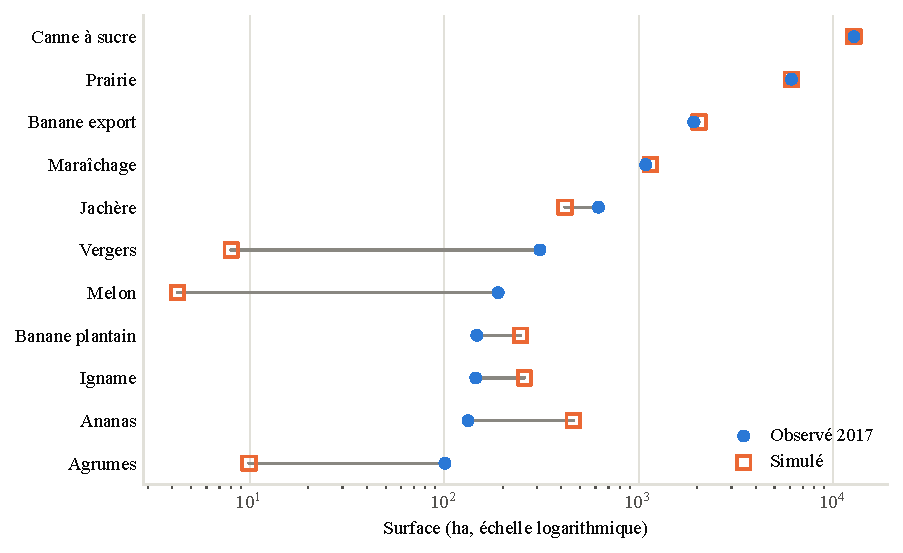
\includegraphics[width=0.88\textwidth]{figures/calibration-observe-simule.pdf}
  \caption{Assolement observé (référence 2017) et simulé (calibration retenue) par groupe de cultures.
  L'échelle est logarithmique et les surfaces vont de \SI{4}{\ha} à \SI{12813}{\ha}.}
  \label{fig:calibration}
\end{figure}


\section{La cause commune de l'écart résiduel : les rendements}
\label{sec:rendements}

La statistique agricole publie, pour chaque culture, une surface et une production, donc un
rendement territorial observé \parencite{agreste2019}. Le tableau~\ref{tab:rendements} le
confronte au rendement que porte l'assolement simulé. L'ordre de grandeur est un facteur
\num{2} à \num{4} sur les cultures diversifiées.

\begin{table}[h]
  \centering
  \caption{Rendement du modèle et rendement du territoire, en tonnes par hectare. La colonne
  Agreste est tirée de la statistique agricole \parencite{agreste2019}. La
  colonne \enquote{modèle} est la production simulée divisée par la surface simulée, mélange
  de variantes techniques compris. Les rendements du modèle sont exprimés \emph{par cycle} et 
  sont donc annualisées avant comparaison.}
  \label{tab:rendements}
  \small
  % Genere par memoire/build_chiffres.py -- ne pas editer.
\begin{tabular}{@{}lrrrr@{}}
  \toprule
  \textbf{Groupe} & \textbf{Agreste 2017} & \textbf{Modèle, par cycle} & \textbf{Modèle, annualisé} & \textbf{Rapport} \\
  \midrule
  Maraîchage & \num{10.8} & \num{43.9} & \num{43.9} & $\times$\num{4.1} \\
  Agrumes & \num{5.2} & \num{20.0} & \num{20.0} & $\times$\num{3.8} \\
  Banane plantain & \num{9.0} & \num{26.0} & \num{26.0} & $\times$\num{2.9} \\
  Vergers & \num{6.4} & \num{14.5} & \num{14.5} & $\times$\num{2.3} \\
  Ananas (18 mois) & \num{12.3} & \num{34.0} & \num{22.7} & $\times$\num{1.8} \\
  Igname & \num{10.0} & \num{17.8} & \num{17.8} & $\times$\num{1.8} \\
  Melon & \num{19.9} & \num{20.0} & \num{20.0} & $\times$\num{1.0} \\
  \bottomrule
\end{tabular}

\end{table}

Une part de cet écart est prévisible. La statistique fait la moyenne de tous les producteurs et
rapporte la production à la surface déclarée. Les jeunes vergers non encore entrés en production
y sont donc comptés. Le modèle, lui, postule le respect des itinéraires techniques et des
rendements tabulés. L'écart vient, en partie, du fait que la statistique agricole publie des
rendements moyens alors que le modèle manipule des rendements potentiels.

Le modèle décrit, pour le maraîchage, une rotation annuelle dans laquelle plusieurs légumes se
succèdent sur le même hectare dans l'année et les récoltes s'additionnent. Au contraire, Agreste
compte une surface par légume et un rendement par légume. Le rapport de \num{\rdtRapportMA}
vient largement de cette méthode comptable.

Le modèle simule la production d'agrumes sur \SI{\simRetenuAG}{\ha}. Son rendement moyen est
donc calculé sur un échantillon de surface restreint, et on essaye de confronter ce chiffre à un
rendement moyenné sur \SI{\obsHaAG}{\ha} observés. Le rapport des deux est donc à ne pas citer
sans ce contexte.

On ne prend pas les données Agreste pour \num{3} raisons :
\begin{itemize}[leftmargin=1.2em,itemsep=3pt]
  \item le respect du mandat de parité, afin de pouvoir attribuer les écarts à des modifications
    déclarées ;
  \item Agreste donne des rendements par culture alors que le modèle donne des rendements par
    itinéraire technique, c'est-à-dire par cultures fines. Avec les données Agreste, le modèle ne
    pourrait pas distinguer deux variantes d'une même culture et on retomberait sur une
    optimisation à \num{12} cultures ;
  \item Agreste sert de juge au modèle, un peu comme le \gls{pad}. On cherche à identifier les
    raisons de l'écart entre le rendement potentiel (modèle) et le rendement réel (Agreste).
    Caler les entrées sur la statistique agricole revient à caler le modèle sur les résultats que
    l'on souhaiterait qu'il produise. Ce serait circulaire et donnerait un modèle surajusté.
\end{itemize}

Le melon est la seule culture du territoire produite presque entièrement par un seul opérateur à
partir d'un unique itinéraire technique. L'écart ne vient pas d'un défaut de données mais plutôt
de la différence entre un rendement potentiel et un rendement moyen. Quand les deux coïncident
comme c'est le cas pour le melon, l'écart disparaît.

Une culture dont le rendement est \num{2} à \num{4} fois trop élevé a une marge \num{2} à
\num{4} fois trop attractive, et le modèle en couvre l'île dès qu'aucun débouché ne la borne.


\section{Deux déviations, et le test qui les sépare d'un ajustement}
\label{sec:deviations}

Toute déviation par rapport à la parité doit avoir une source extérieure au modèle et à
l'observé. L'ajout d'une contrainte à un modèle pour l'approcher du réel doit être justifié. Une
contrainte calée sur l'observé produit mécaniquement un écart nul sur le poste qu'elle vise.
C'est de l'ajustement déguisé en résultat \parencite{howitt1995}. On a retenu \num{2}
déviations.

\subsection*{Première déviation : le plafond de plantain}

Sans contrainte, le modèle donne \SI{\simPariteBC}{\ha} de plantain contre \SI{\obsHaBC}{\ha}
observés. Cela s'explique par la différence de rendement vu précédemment ainsi que par la
contrainte de rotation qui pèse sur son concurrent, la banane. Cela crée, pour le plantain, un
avantage relatif de \SI{4.9}{\percent}. Ce poste correspond pour \SI{20.9}{\mega\euros} à
l'écart d'objectif entre l'optimum et l'observé.

Au lieu de choisir arbitrairement, on a balayé des valeurs de plafond
(annexe~\ref{ann:calibration}). Le balayage donne un palier plat de \SI{4650}{\tonne} 
(plafond donné par l'équation~6 de l'article) jusqu'à \SI{9240}{\tonne}. En dessous de \SI{4650}{\tonne}, 
le plafond devient la production et on contraint explicitement le modèle. Au dessus de \SI{9240}{\tonne}, 
le plafond cesse de mordre et on retombe sur le run de parité avec le plantain à \SI{\simPariteBC}{\ha}.
Entre ces deux bornes, le seuil double pendant que le PAD évolue d'un demi-point, ce qui est à peine plus que le bruit du solveur.
Le plafond n'oblige pas le simulé à coller à l'observé car l'optimum du palier est atteinte pour (\SI{9240}{\tonne}) ce qui est 2,5 fois le débouché observé.
Plus contraignant encore, le modèle freine le simulé mais ne le tire pas vers l'observé. Même 
pour le plafond le plus contraignant, le plantain simulé (247ha) reste supérieur au plantain observé (147ha). 
On choisit finalement un plafond de 6440t. C'est la valeur retenue dans le modèle GAMS.

\subsection*{Seconde déviation : le plancher de prairie}

Ce second cas est gênant, et il faut le dire avant de le défendre : le seuil retenu,
\SI{\mesCalalouBovins}{\ha}, \emph{est} la surface observée. Le \gls{gams} le documente
lui-même — \texttt{QUOTA\_PN\_PIQ\_MIN} y est défini comme la surface 2017 de la prairie au
piquet ; le livre blanc du projet CALALOU relève la même surface bovine ; et le nombre tombe à
\SI{13}{\ha} de notre propre référence parcellaire, qui compte \SI{\obsHaPN}{\ha}. La règle
posée plus haut devrait donc l'interdire. Ce cas demande un test plus exigeant que le plantain,
où le palier plat suffisait.

\paragraph{La nécessité est établie hors du modèle.} Sans plancher, le modèle ne laisse que
\SI{2980}{\ha} à la prairie. L'argument ne passe alors pas par l'assolement mais par le cheptel.
Le territoire portait \num{\mesBovins} bovins en 2017, soit environ \num{\mesUgb} \gls{ugb}
\parencite{agreste2019}. Rapporté aux \SI{\mesPrairieAgreste}{\ha} de prairie de la statistique
agricole, cela fait \num{\mesUgbHaAgreste} \gls{ugb} par hectare, ce que confirment les deux
recensements agricoles encadrant l'année. Rapporté aux \SI{2980}{\ha} du modèle, cela fait
\num{\mesUgbHaSansPlancher} \gls{ugb} par hectare, trois à quatre fois le chargement attesté :
agronomiquement impossible. L'allocation sans plancher n'est donc pas un résultat contre-intuitif
à respecter, c'est un état du monde qui n'existe pas. Le défaut est prouvé sans que le \gls{pad}
soit invoqué à aucun moment.

On pourrait croire que les hectares manquants sont simplement étiquetés sous d'autres cultures.
Ce n'est pas le cas : si les \SI{3489}{\ha} d'écart étaient chez nous rangés en canne, notre
canne dépasserait la statistique agricole, alors qu'elle en restitue \SI{98}{\percent}. Ce sont
donc des parcelles \emph{absentes} de l'univers parcellaire — de l'herbe non déclarée aux aides.
La conséquence est immédiate et elle commande le choix du seuil : ces hectares ne sont pas
récupérables en contraignant l'allocation, puisqu'ils ne sont pas dans l'ensemble de décision.

\paragraph{Ce que la contrainte encode.} Elle n'encode pas l'assolement de 2017, elle encode
une conservation portant sur un stock que le modèle ne décide pas. Le troupeau existe — chiffre
de recensement, indépendant du jeu parcellaire comme du modèle —, il doit se nourrir, à un
chargement attesté. La surface fourragère n'est donc pas une variable libre : elle est déterminée
par une variable d'état extérieure. Tout modèle qui omet l'élevage doit réintroduire cette
détermination de façon exogène, sous peine d'allouer un territoire impossible. La coïncidence
du seuil avec l'observé n'est pas la construction de l'argument mais son résultat : l'exigence
fourragère et l'assolement concordent parce que les éleveurs nourrissent effectivement leur
troupeau, et l'auteur du \gls{gams} a tiré le même nombre du même raisonnement.

\paragraph{Le niveau, par balayage.} La nécessité étant acquise, reste à choisir où placer le
seuil, et à le faire sans se servir de l'ajustement. Le balayage va de \SI{\mesCalalouBovins}{\ha}
à \SI{\mesPrairieAgreste}{\ha}, avec un repère intermédiaire utile : \SI{\mesPrairieExogene}{\ha},
c'est-à-dire la statistique agricole ramenée à la couverture de \SI{\mesCouvertureSau}{\percent}
du jeu parcellaire. Sur toute cette plage, les trois métriques que le plancher ne touche pas
restent au-dessus des seuils publiés par l'article — au plancher le plus haut, encore
\SI{\mesPrairieHautTypes}{\percent} de types, \SI{\mesPrairieHautParcelles}{\percent} de parcelles
et \SI{\mesPrairieHautSurface}{\percent} de surface. En revanche, le \gls{pad} calculé
\emph{hors prairie} \textbf{empire} quand on remonte le seuil, de
\SI{\mesPadHorsPrairieBas}{\percent} à \SI{\mesPadHorsPrairieHaut}{\percent} : le plancher prend
alors sa terre à la canne, c'est-à-dire à la culture que le modèle restitue le mieux et que la
statistique mesure le mieux. C'est le corollaire des hectares absents — forcer la prairie exogène
dans un périmètre trop petit ne peut se faire qu'au détriment du reste. Un seuil choisi pour
flatter le résultat se comporterait exactement à l'inverse.

On retient donc le \emph{bas} de la plage, \SI{27}{\percent} sous les \SI{\mesPrairieExogene}{\ha}
exogènes : le seuil est délibérément sous-contraignant, et il est de surcroît le paramètre du
\gls{gams} d'origine. Ce n'est pas le seuil qu'on défend, c'est la conclusion, et elle ne dépend
pas de lui.

\paragraph{Ce qui n'est pas revendiqué.} Le plancher épingle un quart de la surface cultivée :
le \gls{pad} de la prairie est nul par construction et le \gls{pad} territorial en hérite. Ce
chiffre n'est pas un score (§~\ref{sec:pad}). Il faut aussi se garder d'un argument plus
séduisant : la canne revient à \SI{\simRetenuCS}{\ha} contre \SI{\obsHaCS}{\ha} observés sans qu'aucune
contrainte ne la nomme, mais prairie et canne se disputent les mêmes parcelles, et ce retour est
en partie un effet mécanique de report. C'est un contrôle de cohérence passé — s'il avait échoué,
il y aurait eu un problème —, ce n'est pas une validation indépendante. La justification du
plancher tient au calcul de chargement, pas à l'ajustement qui en résulte.

\paragraph{Pourquoi le modèle perd la prairie.} La décomposition des \SI{3489}{\ha} est en
annexe~\ref{ann:calibration}. \SI{30}{\percent} de la surface perdue tient à un écart de
\SI{0.94}{\percent} entre les marges de deux cultures : à cette échelle, l'arbitrage du modèle
est plus numérique qu'économique. Le reste tient au travail. La Table~1 de l'article donne
\SI{70}{\hour\per\ha} pour la prairie, notre jeu de données \SI{126}{\hour\per\ha}. Ce n'est pas
une erreur de portage : le chiffre n'est lu nulle part, il se recompose depuis l'itinéraire
technique, en multipliant la fréquence annuelle de chaque opération par son temps unitaire —
abreuvement, \num{360} passages de \SI{0.2}{\hour}, soit \SI{72}{\hour} ; déplacement du piquet,
\num{180} $\times$ \SI{0.25}{\hour}, soit \SI{45}{\hour} ; saillies, \SI{6}{\hour} ; traitements
bovins, \num{12} $\times$ \SI{0.25}{\hour}. Sur les sept opérations de l'itinéraire, aucune n'est
un travail du sol : ni labour, ni semis, ni fertilisation, ni fauche. Les deux chiffres ne
comptent donc pas la même chose — l'un le travail de la surface, l'autre le travail du troupeau
qui la pâture, imputé à l'hectare faute d'une variable de cheptel où le loger. Et ces heures
entrent dans le plafond de main d'\oe uvre comme un coût de culture : le modèle paie le troupeau
sans jamais le posséder, ce qui rend la prairie chère sans la rendre rentable.

\paragraph{Le mécanisme manquant.} Le produit animal, lui, est bien présent, mais comme un
coefficient à l'hectare et jamais comme une activité : les tables donnent pour la prairie au
piquet un rendement de \SI{0.66}{\tonne\per\ha} vendu \SI{5000}{\euros\per\tonne}, plus
\SI{550}{\euros\per\ha} de \gls{posei} surfacique. À ce prix, la \enquote{tonne} n'est pas de
l'herbe, c'est de la viande. La marge qui en résulte est d'environ \SI{1602}{\euros\per\ha}, avec
une variance de rendement nulle. L'élevage est donc présent comme produit et absent comme
activité : ni tête de bétail, ni stock, ni report d'une année sur l'autre. Trois conséquences en
découlent. Retirer \SI{3489}{\ha} de prairie, pour le modèle, c'est renoncer à
\SI{1602}{\euros\per\ha} ; dans la réalité, c'est vendre un cheptel, acte irréversible et étalé
sur des années, que rien ici ne pénalise. La variance nulle \emph{aide} la prairie plutôt qu'elle
ne la dessert, si bien que les éleveurs (aversion \num{2.4}) la conservent déjà : recalibrer
l'aversion au risque ne répare donc rien. Et à \SI{1602}{\euros\per\ha} contre
\SIrange{2400}{3500}{\euros\per\ha} pour la canne mécanisée, la prairie perd légitimement
l'arbitrage — le modèle a raison dans ses termes, ce sont ses termes qui sont incomplets. Ce qui
manque n'est pas un prix mais une variable d'état, celle qui interdirait de liquider un troupeau
gratuitement, et que \textcite{chopin2015} reconnaît comme sa propre limite.

Cette lecture donne au plancher son statut exact. Il n'est pas un correctif provisoire ajouté au
jugé : il est la \emph{forme réduite} d'une équation qui n'est pas implémentée — surface
fourragère supérieure au cheptel divisé par le chargement — évaluée au troupeau de 2017. Le
modèle complet ferait de l'\gls{ugb} une variable de décision, du chargement un levier, et de la
marge de la prairie une fonction de la densité animale au lieu d'une constante. Tant qu'il
n'existe pas, le cas dégénéré à cheptel fixé est le meilleur substitut disponible, et il est
exact pour l'année simulée. Cela délimite aussi ce que le modèle ne peut pas explorer : aucune
question portant sur l'intensification de l'élevage, puisqu'il ne sait pas arbitrer entre moins
de surface plus chargée et plus de surface extensive. En prospective, le seuil doit alors être
lu pour ce qu'il est — une hypothèse de cheptel — et se déclarer comme telle dans chaque
scénario plutôt que rester une constante héritée (§~\ref{sec:deviations} et chapitre~4).

\subsection*{Le coût des deux déviations}

Les deux contraintes adoptées coûtent \SI{0.7}{\percent} de l'objectif pour le plancher de
prairie et \SI{3.7}{\percent} pour le plafond de plantain. Un troisième levier a été envisagé et
non retenu, le plancher arboricole, dont le coût mesuré va de \SI{0.39}{\percent} à
\SI{200}{\ha} à \SI{1.19}{\percent} à \SI{335}{\ha} ; il a été écarté parce que les runs qui le
portaient atteignaient la limite d'une heure avec un incumbent incohérent, donc inexploitable.
Les deux corrections retenues sont du même ordre de grandeur que ce candidat : aucune n'est une
correction massive imposée au modèle. Elles corrigent, elles ne réécrivent pas.

\subsection*{Une contrainte que l'on n'a pas posée}

\SI{430}{\ha} d'ananas intensif apparaissent chez les canniers et les bananiers, et aucune
contrainte actuelle ne l'interdit. Ce que le modèle vérifie sur une exploitation tient en deux
lignes : des hectares éligibles et un total \emph{annuel} d'heures de travail. Ces
\SI{430}{\ha} passent les deux tests. Ce qu'un agronome regarderait, le modèle ne le porte pas.
Le calendrier d'abord : le cycle de l'ananas dure \num{\mesCycleAnanas} mois quand le modèle est
mono-période annuel, et une exploitation cannière a déjà ses pointes de plantation et de récolte
dont un total annuel ne dit rien. Le matériel végétal ensuite : l'ananas se plante par rejets
issus des plantations existantes, et \SI{430}{\ha} supposent un stock qui n'existe pas sur le
territoire et met plusieurs cycles à se constituer. L'équipement et le savoir-faire enfin : une
exploitation cannière possède des machines de canne et une main d'\oe uvre formée à la canne,
quand le modèle n'a ni capital, ni compétence, ni coût d'apprentissage — changer de culture y est
gratuit et instantané. Le débouché, pour finir, est une filière organisée qui n'absorbe pas
\SI{430}{\ha} supplémentaires par construction.

Ce n'est donc pas une erreur de calcul mais une contrainte manquante, de la même famille que
l'élevage : le modèle ignore qu'un métier ne se change pas en une saison, et rien dans ses
sorties ne le signale. Le résultat reste plausible tant qu'on ne regarde pas qui cultive quoi.

\section{Explications de l'écart résiduel}
\label{sec:plateau}

La résolution n'est pas responsable de l'écart résiduel. L'hypothèse qu'il existerait un
meilleur optimum que le solveur n'a pas trouvé est fausse (§~\ref{sec:tractabilite}).

La situation observée de 2017 donne un objectif de \SI{\mesPlanObserveM}{\mega\euros} alors que
l'optimum est de \SI{\mesPlanOptimumM}{\mega\euros}. Cette écart de \SI{\mesPlanEcart}{\percent}
correspond à \num{15} fois la tolérance d'optimalité imposée au solveur. On peut donc dire que
le modèle converge bien mais qu'il ne maximise pas la même chose que les agriculteurs.

De plus, \num{3} optimisations de même configurations donnent \SI{\mesGraineA}{\percent},
\SI{\mesGraineB}{\percent} et \SI{\mesGraineC}{\percent} de \gls{pad}. L'arbitraire du solveur
vaut \SI{\mesBruitPad}{\percent} de \gls{pad} et c'est ce chiffre qui fixe la tolérance des
garde-fous du dépôt (§~\ref{sec:gardefous}).

Concernant la main d'\oe uvre, la situation observée demande \SI{\mesMoObserve}{\mega\hour} pour
un plafond de \SI{\mesMoPlafond}{\mega\hour}. Le plafond n'interdit pas l'assolement réel.

La recalibration sur 2017 des coefficients d'aversion au risque donne un \gls{pad} de
\SI{39.9}{\percent} mais au prix d'un surajustement qui rend les coefficients économiquement
absurdes. La piste est abandonnée.

Caler des plafonds de marché sur l'observé descend à \SI{33.6}{\percent}, et c'est circulaire
par construction, puisque la contrainte est l'observé. La piste est abandonnée.

Implémenter l'élevage semble être la bonne piste mais c'est un chantier important. Il a donc été
écarté ici plutôt que bâclé. Il correspond à la seconde partie du stage qui n'est pas encore
réalisée et \textcite{chopin2015} reconnaît son absence comme sa propre limite.

\section{Deux signatures émergentes}
\label{sec:emergence}

La canne à sucre est à \SI{\simRetenuCS}{\ha} contre \SI{\obsHaCS}{\ha} observés
(\SI{\padRetenuCS}{\percent} de \gls{pad}) sans qu'aucune contrainte ne la nomme. Le modèle,
laissé entièrement libre sur la culture qui occupe plus de la moitié du territoire, retombe sur
l'observé.

De même, la banane revient sous le plafond de plantain, et la canne sous le plancher de prairie.
Pour ces deux cultures, le modèle se rapproche de l'observé grâce à des contraintes agissant sur
d'autres postes. Cela semble indiquer que la structure économique du programme est juste,
indépendamment des seuils qu'on lui impose.

Sur l'arboriculture, le modèle est plus proche de la statistique agricole que de notre propre
référence parcellaire. L'écart mesuré est en partie un écart entre la référence et la réalité ce
qui relativise la responsabilité du modèle dans ce cas précis. À noter que le déficit
d'arboriculture ne vient pas de l'inéligibilité mais du rendement horaire. Avec un plafond de
main d'\oe uvre, ce qui compte n'est pas la marge à l'hectare mais la marge à l'heure.

\begin{reflexion}
réflexivité
\end{reflexion}
